% Version history:
% $Log$
% Revision 1.1.2.7  2005/03/06 11:10:14  kelsaka
% finished adding content
%
% Revision 1.1.2.6  2005/03/05 16:06:57  kelsaka
% added content
%
% Revision 1.1.2.5  2005/03/04 16:16:44  kelsaka
% added content
%
% Revision 1.1.2.4  2005/03/04 08:17:46  kelsaka
% added further content
%
% Revision 1.1.2.3  2005/03/03 16:36:43  kelsaka
% reviewed and corrected original text from the tech report; added updated graphics
%
% Revision 1.1.2.2  2005/03/02 17:26:15  kelsaka
% added images; started english texting...
%
% Revision 1.1.2.1  2005/02/20 13:17:04  kelsaka
% erste Inhalte hinzugef�gt
%



\documentclass[a4paper,12pt]{article}
\usepackage[latin1]{inputenc}
\usepackage{graphicx}
\usepackage[left=2.5cm,right=2.5cm,top=2.5cm,bottom=2.5cm]{geometry}
\setlength{\baselineskip}{1.5\baselineskip}



	

\title{The Palladio Component Model}
\author{Palladio Research Group,\\
Fk. II, Department f�r Informatik,\\
Carl-Von-Ossietzky Universit�t Oldenburg}
\date{\today}




\begin{document}
\maketitle


%\vspace{3cm} %causes toc to take more than the first page.
\tableofcontents

\newpage
% \pagenumbering{arabic} %%numbering in the header
\pagestyle{headings}




% ############################
\section{Overview}
\label{sec:Overview}
The Palladio component model is the meta-model for specifying component models in the context of the Palladio framework. Currently the specification of a layered logical view on basic components, components built by assembling components and component connections is supported. To gain a better understanding of the model take a closer look at figure \ref{fig:componentmodel}.

As already mentioned the component model is multi-layered. It differs between a type-, implementation-, and deployment-layer to allow realistical modelling of software-systems. To give an easy introduction first the general elements (mainly at the type-level) are described.


\begin{figure}[htb]
	\centering
		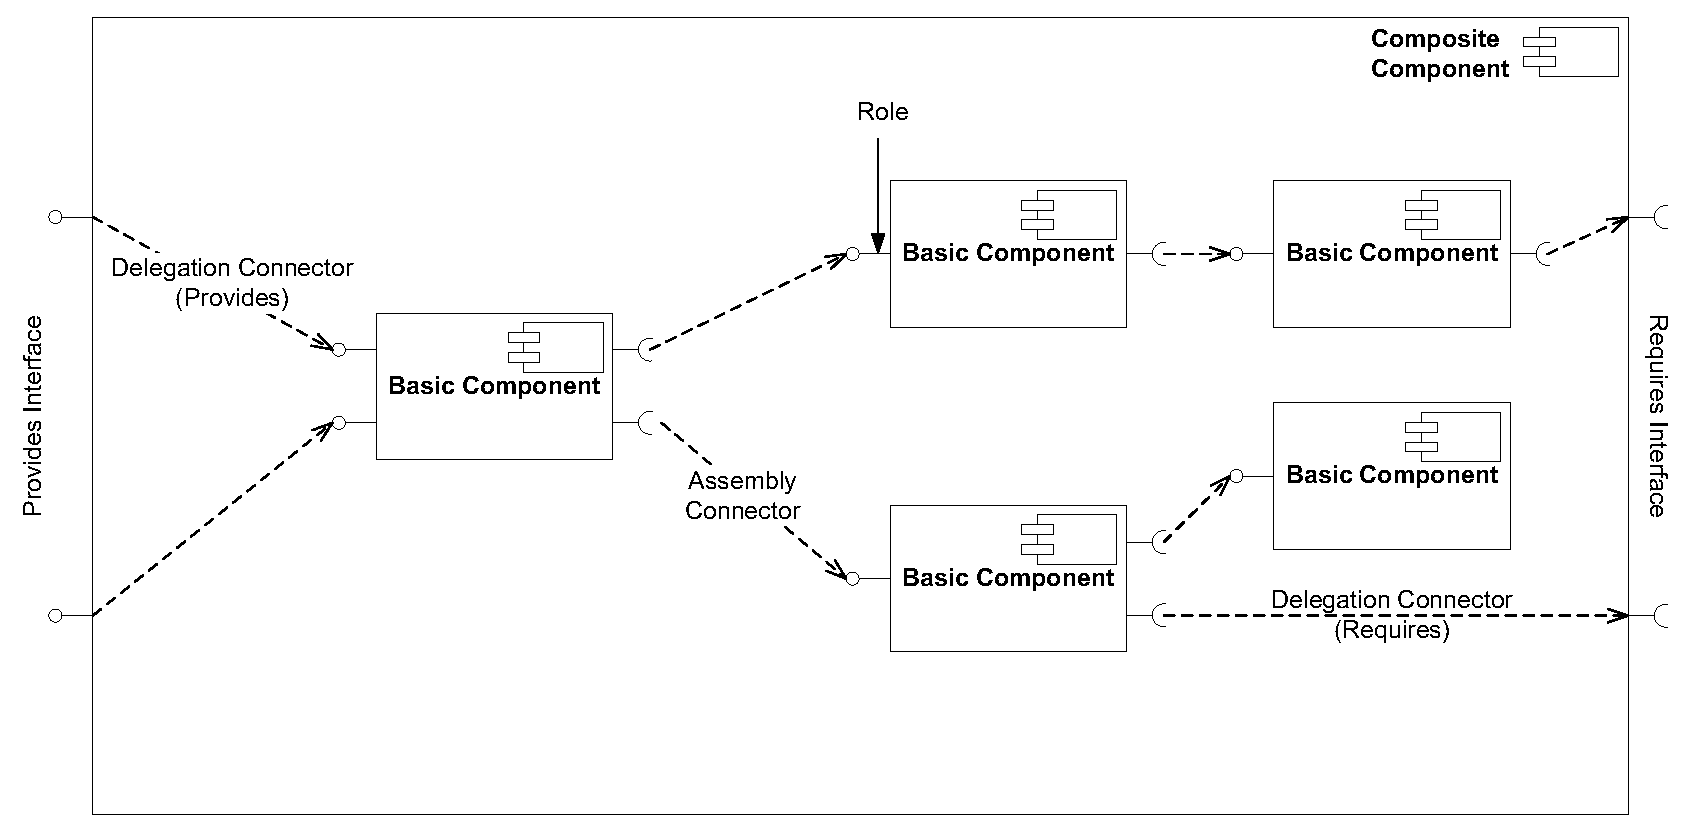
\includegraphics[width=1.00\textwidth]{images/architectural-blocks01.pdf}
	\caption{Building blocks of the Palladio component model}
	\label{fig:componentmodel}
\end{figure}


\subsection{Components}
As depicted a component can be of two different types. 
\begin{itemize}
\item \emph{Basic Component}: A basic component can be seen as a black box entity for the component based system. There is no additional knowledge of the internal structure of those components, e.g. whether they are build from other components or not. A basic component is characterized by its interfaces as described later on.
\item \emph{Composite Component}: A composite component is a container for other components (basic or composite). It is supposed to offer a set of interfaces belonging together, e.g., by fulfiling a complete domain task. The components which are part of a composite component are wired internally by so called connections which again are introduced later. Composite Components are just logical enitities with no physical representation.
\end{itemize}

\subsection{Roles and Interfaces}
A component has a two sets of interfaces. A set of provides interfaces, where the services the component offers to the environment are located, and a set of requires interfaces, containing all the services needed from the environment in order to operate correctly. In order to identify a single service uniquely an interface provided or requires of a component is called a role and given a role identifier. For example, imagine a service called aService offered by two provides interfaces of the component. The first interface has the role identifier A and the second one B. Then it becomes possible to identify those services by writing A.aService and B.aService. The term "Role" comes from the role the component plays in an interaction with its environment when referring to single service calls.

An interface is described by a so called \emph{interface model}. The interface model is a container for the information that can be associated to the interface. As a minimum requirement the interface model always consists of a list of signatures stating the provides- or required services respectively. Additionally, any kind of \emph{auxiliary information} can be attached to an interface, like protocol information using FSMs (see section \ref{sec:protocols}) or petri-nets. Other possible information can be thread safety specifications, logical constraints (pre- and postconditions) or even domain related QoS aspects. The actually needed auxiliary information is depending on the analysis one wishes to perform on the specified model.


\subsection{Connections}
The basic components and their interfaces are inter-connected in a composite component by two different types of connectors. The visualisation refers to the UML 2.0 connectors (see \cite{carnegie}).

\begin{itemize}
\item \emph{Assembly Connector} (aka Binding): This kind of connection is used to connect a requires interface of one component to the provides service of another component. Such a connection has the meaning that any call of the requiring component to the respective requires role is actually redirected to a call of an appropriate provided service on the providing component. Note that there might be some kind of connector involved in this process, like using a RMI or .NET Remoting call.

\item \emph{Delegation Connector} (aka Mapping): Delegation connectors are logical constructs which map the provided or required services of the composite component to contained components. A delegation connector maps a component's external behavior to an internal realization of that behavior by one of its sub-components. 

There are two types of delegation connectors: \textit{Provides delegation connectors} are used to map provides services to components offering those services and \textit{requires delegation connectors} are used to map required services to requires interfaces of the composite component.


\end{itemize}

The different types of connections can be seen in figure \ref{fig:componentmodel} and figure \ref{fig:connections} respectively.

\begin{figure}[htb]
	\centering
		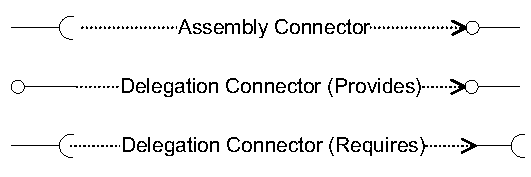
\includegraphics[width=0.60\textwidth]{images/connections01.pdf}
	\caption{Different types of connections}
	\label{fig:connections}
\end{figure}

Note, that if you imagine an additional requires or provides interface respectively for the mappings then a (general) connection can be seen as a link between a requires and a provides role.

Formally a connector is just a link between two interfaces. It is not a real own entity. (TODO: emphasize that there is nothing that connects interface and connector)



\subsection{Service Effect Specification}
The Palladio component model supports the specification of so called \emph{service effect specifications} (SEFF). A service effect specification is a description of the behaviour of a single service - restricted to external interaction, i.e., if service A calls service B and C then B and C are part of the service effect specification of service A. In general the specification is represented by a finit state machine (FSM).

The service effect can be seen as a special kind of interface model that is defined by the component that implements a interface. In fact not a interface has the service effect specification but a component implementation has a specification for each service provided. Chapter ref{TODO} shows at which level of the component model service effect are specified.

The main difference between an interface and a service effect specification is the type of the signatures used in the specification. With respect to the service effect specification a role identifier needs to be added to a signature to identify the external services uniquely, e.g., consider a service calling "save" on a file and on a database simultaneously. Then, in order to differentiate both of them the role identifier like "DatabaseStore" and "FileStore" are needed. This difference is not needed for interface specifications, as a signature is already identified by the interface offering the respective service.

An example of a service effect specification consisting of the external signatures and their calling order specified as FSM is depicted in figure \ref{fig:serviceeffect}.

\begin{figure}[htb]
	\centering
		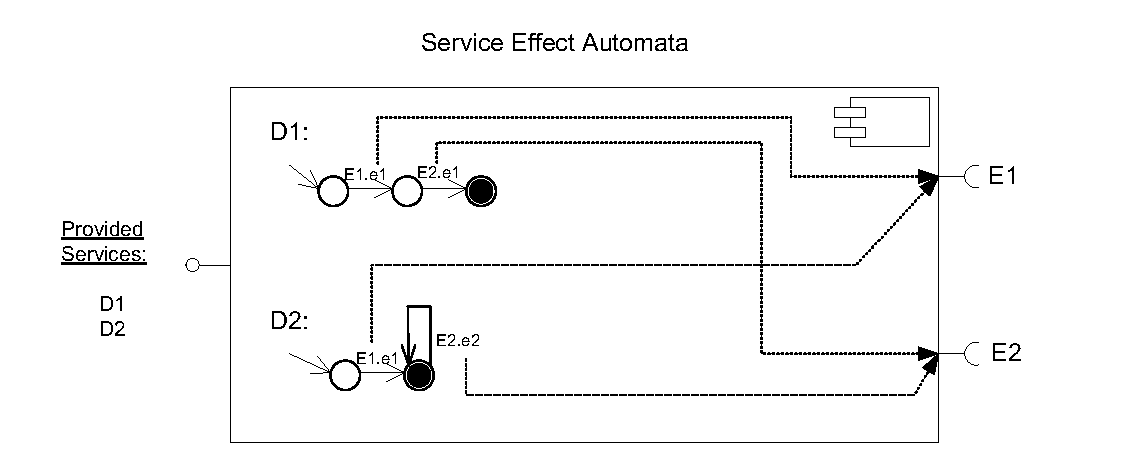
\includegraphics[width=1.00\textwidth]{images/service-effect01.pdf}
	\caption{Example service effect specification}
	\label{fig:serviceeffect}
\end{figure}



\subsection{Protocols}
\label{sec:protocols}
Interface protocols mostly are described using FSMs. They are attached to interfaces as additional attributes and describe all correct orders of calling services, either at the provided or required side.

\subsubsection{Provides Protocol}
The \textit{provides protocol} describes in which order the provides services have to be called, to use a interface properly. E. g. a typical access to a filesystem has a calling sequence like
\[
OpenHandle()\ \ (\:Read(),\ Write()\:)^{+}\ \ CloseHandle()
\]
as regular expression. Visualized as a FSM this protocol looks like depicted in figure \ref{fig:providesProtocol}.
\begin{figure}[htb]
	\centering
		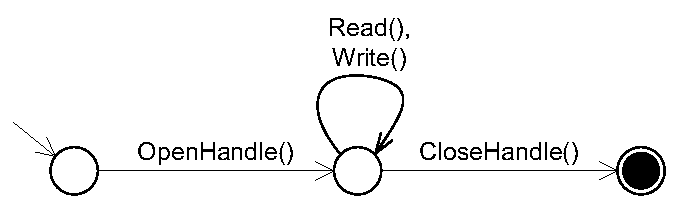
\includegraphics[width=0.50\textwidth]{images/provides-protocol01.pdf}
	\caption{Example provides protocol}
	\label{fig:providesProtocol}
\end{figure}


\subsubsection{Requires Protocol}
The \textit{requires protocol} describes in which order external services, that are generally given by the service effect specification, are called. So requires protocols extract the calling-orders on \textit{one} interface out of the service effects, while the service effect specification defines a order of calls on a \textit{number} of interfaces. This means that mostly requires protocols are calculated. (TODO: completely understood?)


\subsection{Resources}
Resources are special entities for the deployment level of architectural modelling (see section \ref{sec:layeredModel}). They describe hardware-environments in the model.

\begin{itemize}
\item \emph{Computational}: A developed software-system uses this kind of resources for computing values and processing information. E. g. this are processors, virtual machines or even operating systems.

\item \emph{Non-Computational}: Part of this class of resources are router, switches, network-cables, internet-connections. Software does not use this resources to compute, but for connection activities.
\end{itemize}


\subsection{First Class Entities}
The component model offers three types of \textit{first class entities}. They may exist without being connected or attached to the rest of a model. Basic Components, Interfaces and Ressources (see section TODO) are first class entities. E. g. this means it is possible to have multiple interfaces that are not connected to any components, as interface can exist by there own.


\subsection{Multiple Occurrences and Identity}
All entities in the component model have Globally Unique Indentifiers (\textit{GUID}s) to be able to decide whether they are identical or the same. This permits the modeller to name components and interfaces the same though different entities are meant. The following entities are equiped with GUIDs: Interfaces, Basic Components, Composite Components, Resources, Roles, Attributes, and ...TODO.

To allow easy modelling of software architectures entities may occur multiple times. Due to the use of GUIDs e. g. interfaces can occur attached to several components at the same time. As \textit{one} interface in fact often is implemented by a lot of components a graphical representation of the model stays more clearly arranged. And as well attributes of an interface can be changed centrally. Figure \ref{fig:GUID01} shows an simple example of the use of GUIDs.

\begin{figure}
	\centering
		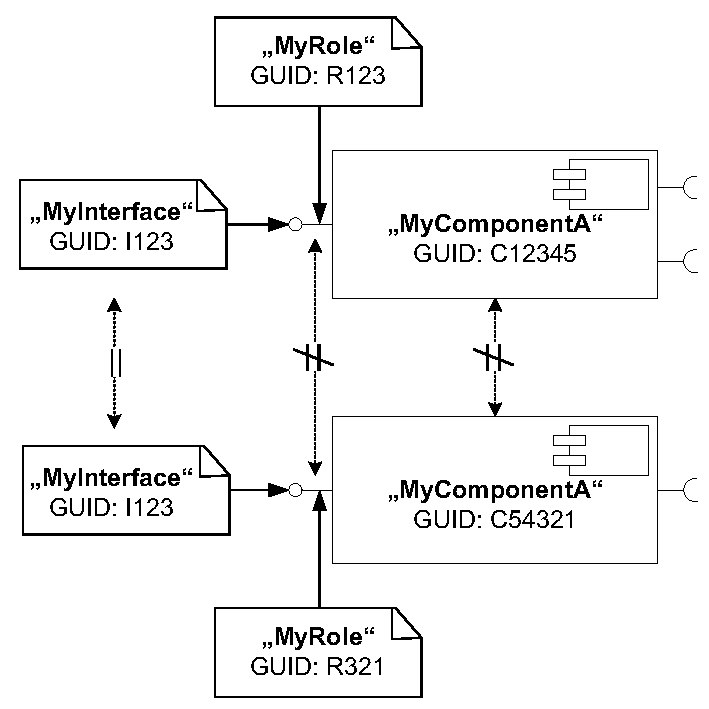
\includegraphics[width=0.50\textwidth]{images/GUID01.pdf}
	\caption{Use of GUIDs in the component model}
	\label{fig:GUID01}
\end{figure}





% ############################
\newpage

\section{Layered Model}
\label{sec:layeredModel}


\subsection{Layers}
\label{sec:layers}
For being able to model realistical component based software systems the component model is split into three layers: the type-level, the implementations-level, and the deployment-level. This way it is possible to differ between component-types, their implementation or their deployment. In constrast to former versions of the component model the implicit limitation to 1:1:1-relations between the layers was removed by modelling the layers explicitly. Which means the possibility of modelling \textit{n} implementations for \textit{one} type and \textit{n} deployments for \textit{one} implementation. Figure \ref{fig:meta-scheme-implementation-layers01} shows the mulitpicities between the layers.


\begin{figure}[ht]
	\centering
		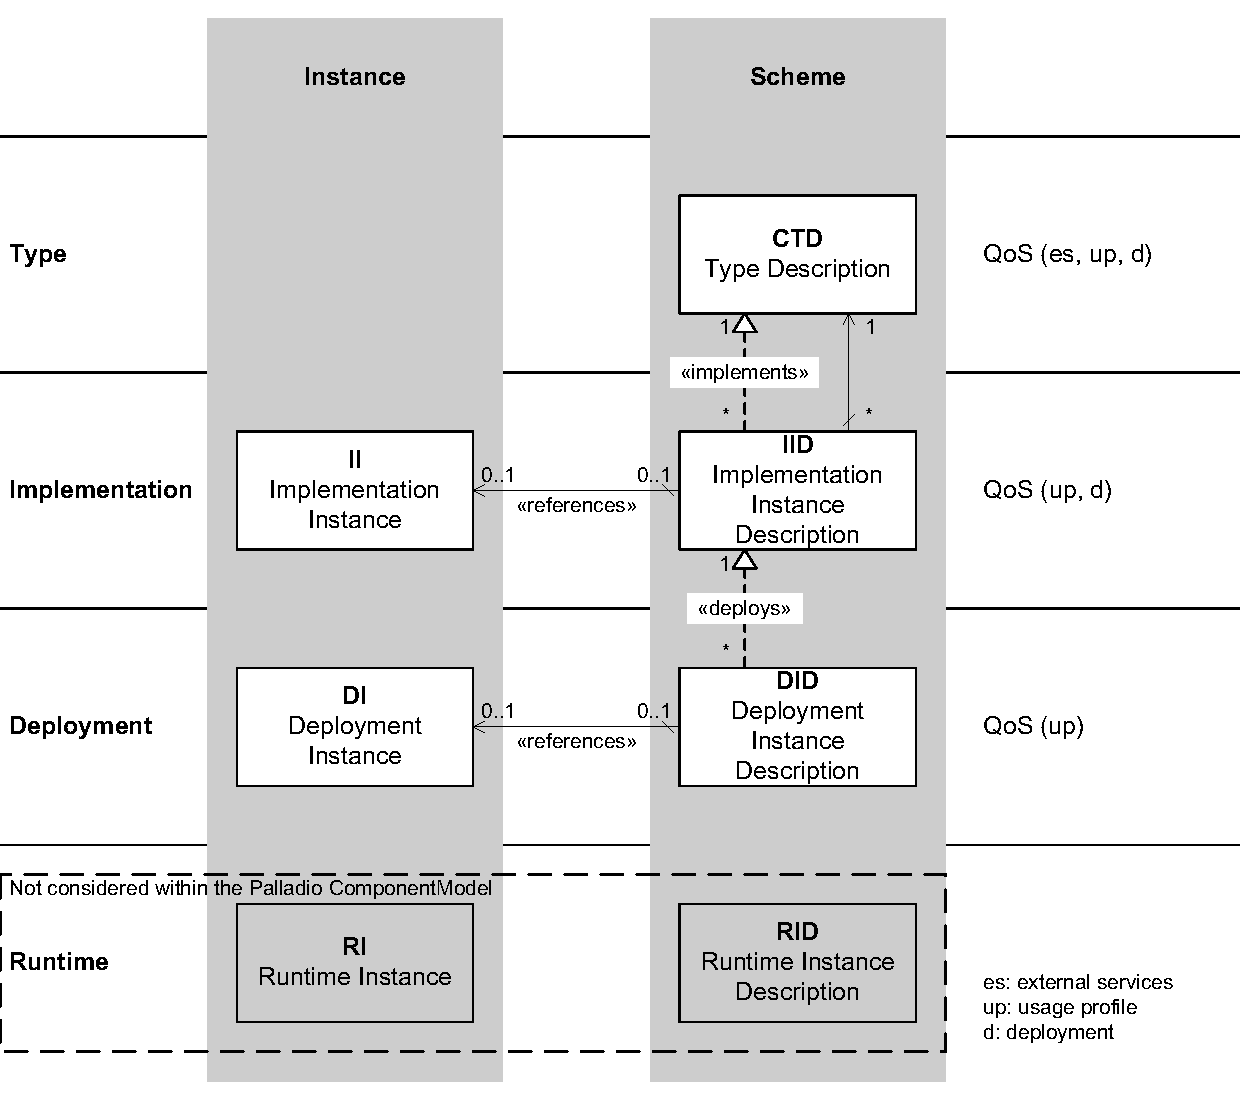
\includegraphics[width=1.00\textwidth]{images/meta-scheme-implementation-layers01.pdf}
	\caption{Instance- and scheme-assignments at the detail-levels}
	\label{fig:meta-scheme-implementation-layers01}
\end{figure}
 
Figure \ref{fig:meta-scheme-implementation-layers01} describes the layers of the component model. The main seperation into \textit{type}, \textit{implementation}, and \textit{deployment} is depicted vertically. To keept the complexity of the model handleable the \textit{runtime-level} is not modelled. Anyway it is possible to include runtime-information by assuming a 1:1-relation between the deployment- and runtime-level. This means, that each deployed component implicitly has exactly one runtime-instance. Runtime-informations have to be put to the deployment-level. Therefore only systems can be modelled that do not have duplicated runtime instances of a component.

Horizonally the component model differs between scheme and instance of a component or interface. At the implementation-level the implementation description may contain a reference to a code artefact. To allow easy modelling a description can exist without a concrete implementation as well as a implementation without a description is supported. Sourcecode written in a different programming language or a compiled version of code always has its own description (note the 0..1 to 0..1 relation, as shown in figure \ref{fig:meta-scheme-implementation-layers01}). Depending on the programming language different descriptions are possible, whose symmetric difference (TODO: symmetrische Differenz) is not empty (e. g. if the programming languages support different constructs). So there would be not meaningful common description.

Navigating at the horizonal axis generally only works from the description, using the contained reference, to the implementation.

In the same way the description of the deploymentinstance has a reference to the deploymentinstance and the navigation is limited to direction from description to instance.

The type-level has no instance because it is a mere modelling-level with no physical representation. Because of this \textit{CompositeComponents} are covered by this level, as they \textit{logically} encapsulate a set of components and their provided and required interfaces.



\subsection{Quality of Service}
\label{sec:QoS}
Quality of Service (QoS) Attributes at the \textit{type-level} depend on the following parameters:

\begin{itemize}

\item The used \textit{external service}. These services are not set by the type-description, as the implementation fixes how functionality is realised. At the type-level the used external services are not defined.

\item The \textit{deployment} of the components. It is not commited which hardware-environment is available for computing.

\item The \textit{usage profile}. This parameter allows dependencies on the scenario in which a component is used. E. g. even load or peak loads can be modelled.

\end{itemize}

The more concrete a modelling-level gets, the less model-space (TODO?) is available for QoS-attributes. The \textit{implementation-level} depends on the deployment and the usage profile, whereas the \textit{deployment-level} only depends on the usage profile. At the runtime-level, which is not explicitly modeled, the QoS-Values have no parameters and can be dertermined exactly.



\subsection{Modelling}
\label{sec:Modelling}
The supposed direction of modelling is top-down. This procedure corresponds to a consecutive refinement of the specification. The type-level has to be designed before the implementation- and deployment-level can be added. Like figure \ref{fig:attributes-example01} shows, attributes are inherited lower levels.

If the next lower level is specified in the model, it is first initiated with inherited attributes. In the following step they can be modified. This modelling decision is based on the assumption, that implementations and deployments mostly fit excatly to their higher specification level.

The language usage for the inheritance relation from the implementation- to the type-level is characterized with the $\ll$implements$\gg$ stereotype. The relation between the deployment- and implementation-level is called $\ll$deploys$\gg$.



\subsection{Attributes}
\label{sec:Attributes}

\begin{figure}[htbp]
	\centering
		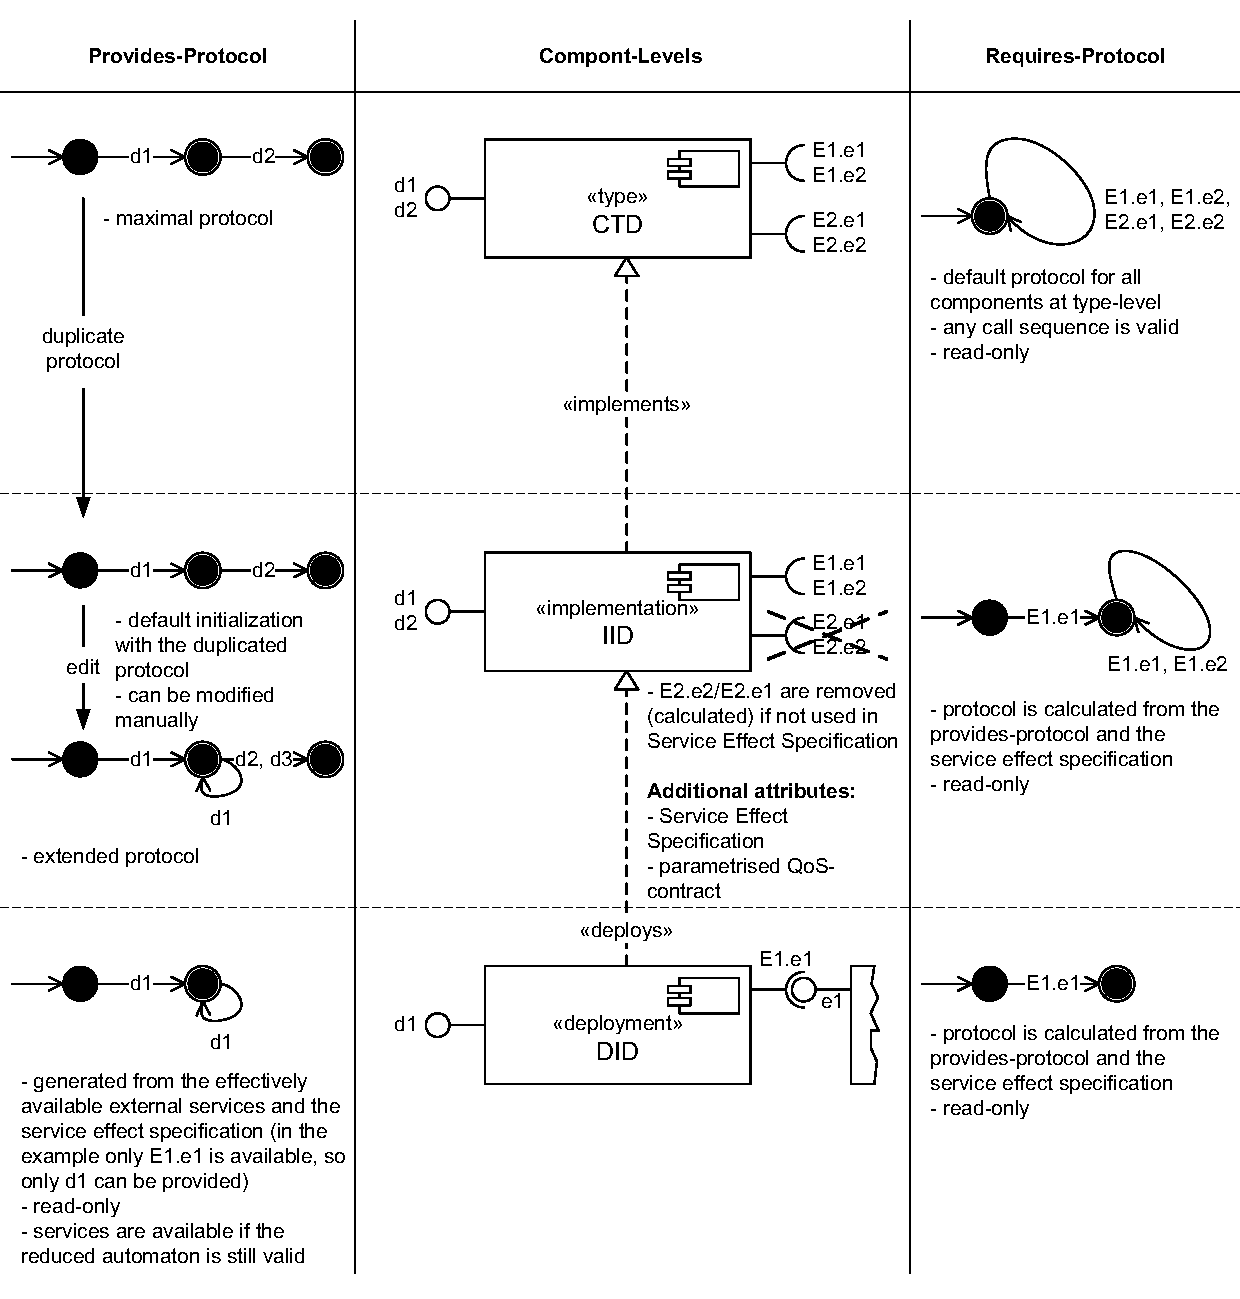
\includegraphics[width=1.00\textwidth]{images/attributes-example01.pdf}
	\caption{Example model including possible attributes}
	\label{fig:attributes-example01}
\end{figure}

Between the layers of component specification attributes are inherited top-down (see figure \ref{fig:attributes-example01}). This means, that attributes that are given at a higher level are also available for lower levels. According to the usual understanding of inheritance (in software) lower layers can add attributes.



\subsubsection{Provides-Protocol}
At the \textit{type-layer} always a maximal protocol is defined. This protocol initially is duplicated for the \textit{implementation-layer}. Afterwards it may be \textit{extended} (e. g. using additional states and transitions like the "d1" transition in the example, figure \ref{fig:attributes-example01}). However the subtype-relation has to be fulfilled. Therefore at the type-level implementation-descriptions of the same type-description can be replaced with each other.

At the \textit{deployment-level} the provides-protocol can not be modified manually, it is read-only. The effective provides-protocol is calculated from the available external services and the SEFF. If for a provided service not all external used services from the SEFF are available, because not all requires-interfaces are fulfilled, the provided services from the considered component are reduced. Only services, whose external service calls from the SEFF are fully available, can be provided. Thus only these services appear in the provided signature list and the provided protocol. So at the deployment-level components can be connected, that do not have a fully fitting protocol or signature list.

Just correct partial automatons (TODO: Teilautomat?) (which are calculated by the procedure described above) of the provides-protocol from the implementations-layer are valid provides automatons at the deployment-level. If the calculations leads to no valid partial automaton (TODO) (the accepted language of the automaton: $L(A) = \emptyset$) no services can be offered.



\subsubsection{Requires-Protocol}
At the \textit{type-level} a trivial requires-protocol is assumed. It allows any order on calling external services (see figure \ref{fig:attributes-example01}). This protocol is read-only and the default protocol for all interfaces at the type-level.

At the \textit{implementation-level} the requires-protocol is calculated from the provides-protocol and the SEFF. The calculation can be sketched (for FSMs):
\begin{itemize}

\item for all transitions (services) in the provides-protocol get into the SEFF, that describe the called service.

\item for the new requires-protocol: expand the just viewed transition from the provides-protocol with all transitions from the SEFF.

\item assuming that $\varepsilon$-transitions are used, the initial state from the SEFF gets connected (with a $\varepsilon$-transition) with the previous state from the provides-protocol.

\item final states from the SEFF get non-final. They have to be connected to the following state from the provides-protocol (with a $\varepsilon$-transition).

\end{itemize}


The calculation is illustrated in figure \ref{fig:requires-protocol01}. In the example a automaton with $\varepsilon$-transitions is created. At all the requires-protocol is the provides-protocol extended by the service effect specifications. This leads to quite a big automaton. 

\begin{figure}[hpbt]
	\centering
		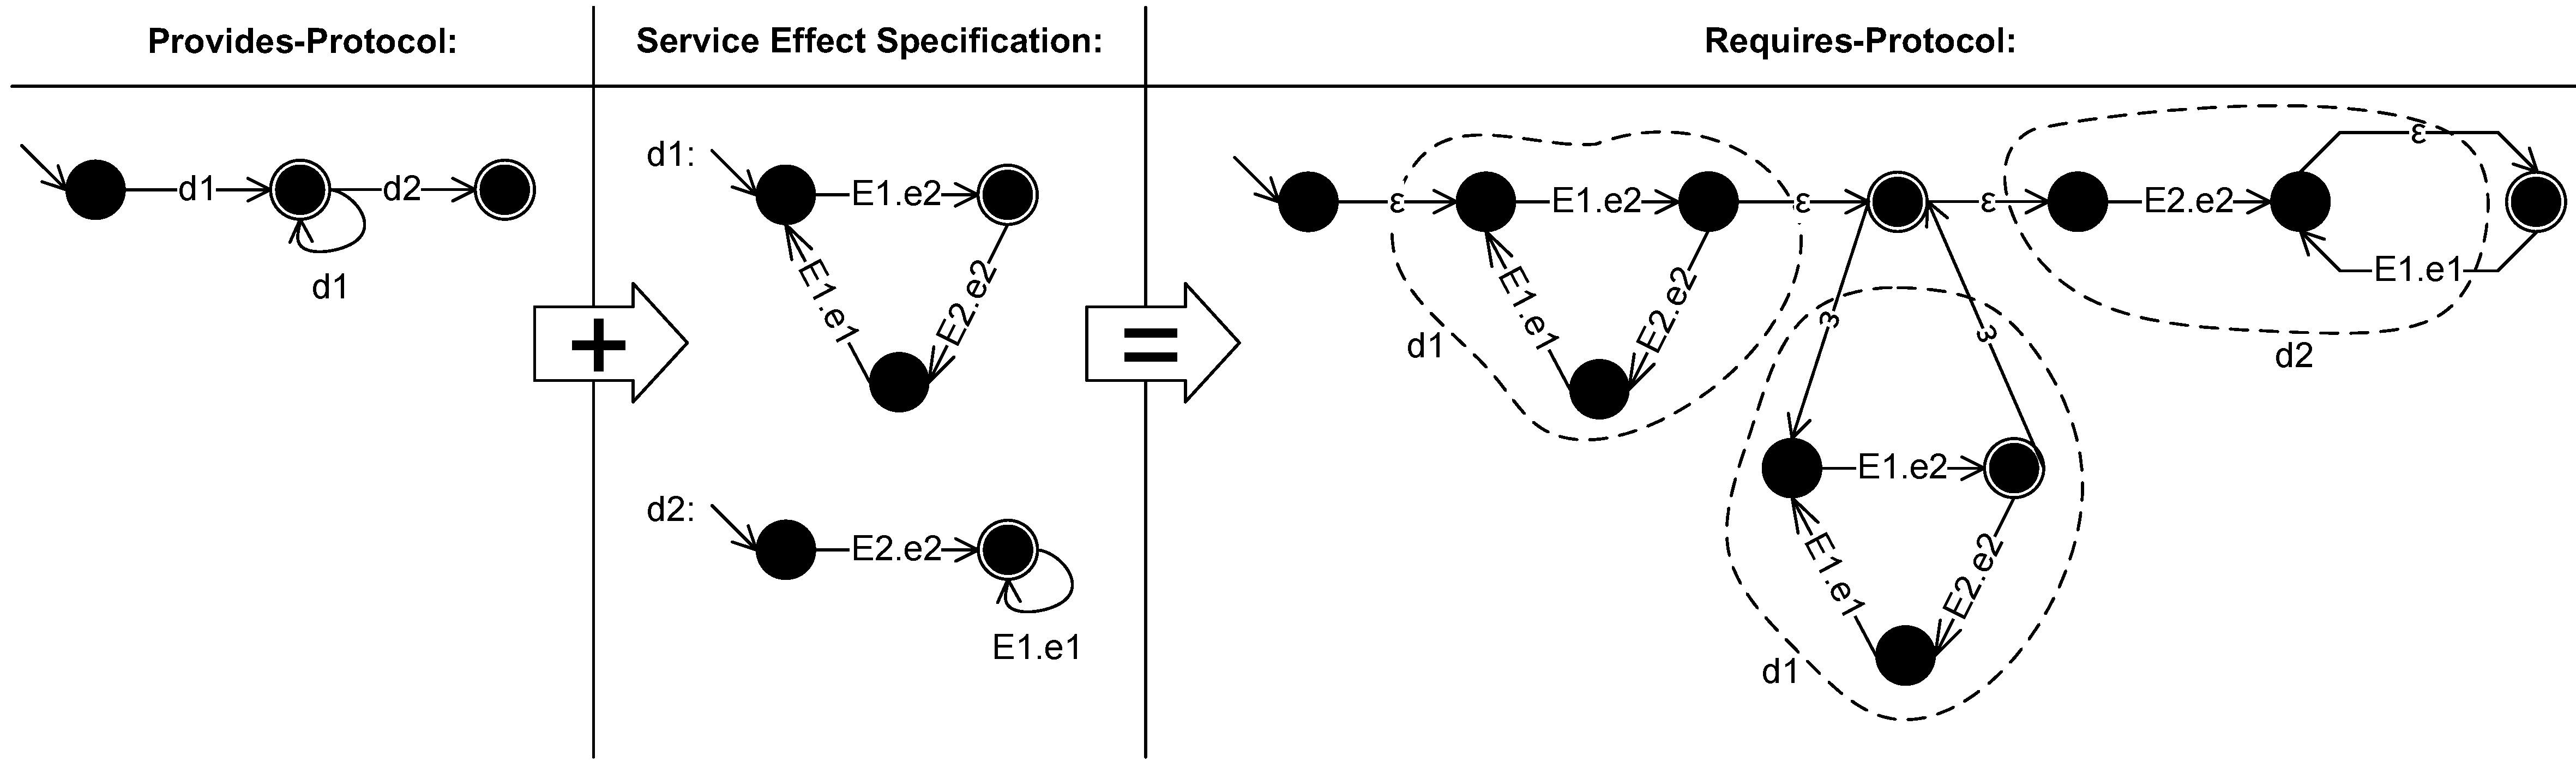
\includegraphics[width=1.00\textwidth]{images/requires-protocol01.pdf}
	\caption{Example: calculating a requires-protocol}
	\label{fig:requires-protocol01}
\end{figure}

As the requires-protocol allows any calling-sequence at the type-level the requires-protocol at the implementation-level is a limitation of sequences. For the languages of the automatons the following relation has to be valid, with language at type-level $L(A_{type})$ and language at implementation-level $L(A_{implementaion})$
\[
L(A_{type}) \ \subseteq \ L(A_{implementaion}).
\]
The requires-protocol at the implementation-level is read-only.

At the \textit{deployment-level} the requires-protocol is calculated in the same way like at the implementation level. It is read-only, too. Since the protocol is calculated from a reduces provides-protocol it may be reduced as well.



\subsubsection{Additional Attributes}
Generally all attributes are inherited top-down. Descriptions from a lower level are specialisations from higher levels. Attributes from the type- to the imlemetation-layer have to fulfill the requirements for subtyping. So attributes may change from level to level but they have to keep consistence.

Type- and implementation-level follow the co- / contra-variance principle, that is known from programming languages like Java, C++ or C\#. This allows to model as known from these languages including subtype relations.

In contrast to the first two layers the deployment-level allows to reduce attribute values or contracted attributes. By supporting this behaviour very dynamical architectures can be created, where components are exchanged. The newly created architecture can be examined, although the requires-interface it not completely fulfilled. As well components can be connected to requires-interfaces though they do not provides all required services. Please note that a component's implementation has to support such a kind of fault-tolerance. Otherwise errors might be caused.



\subsection{Visualization}
\label{sec:Visualization}

\begin{figure}[p!tbh]
	\centering
		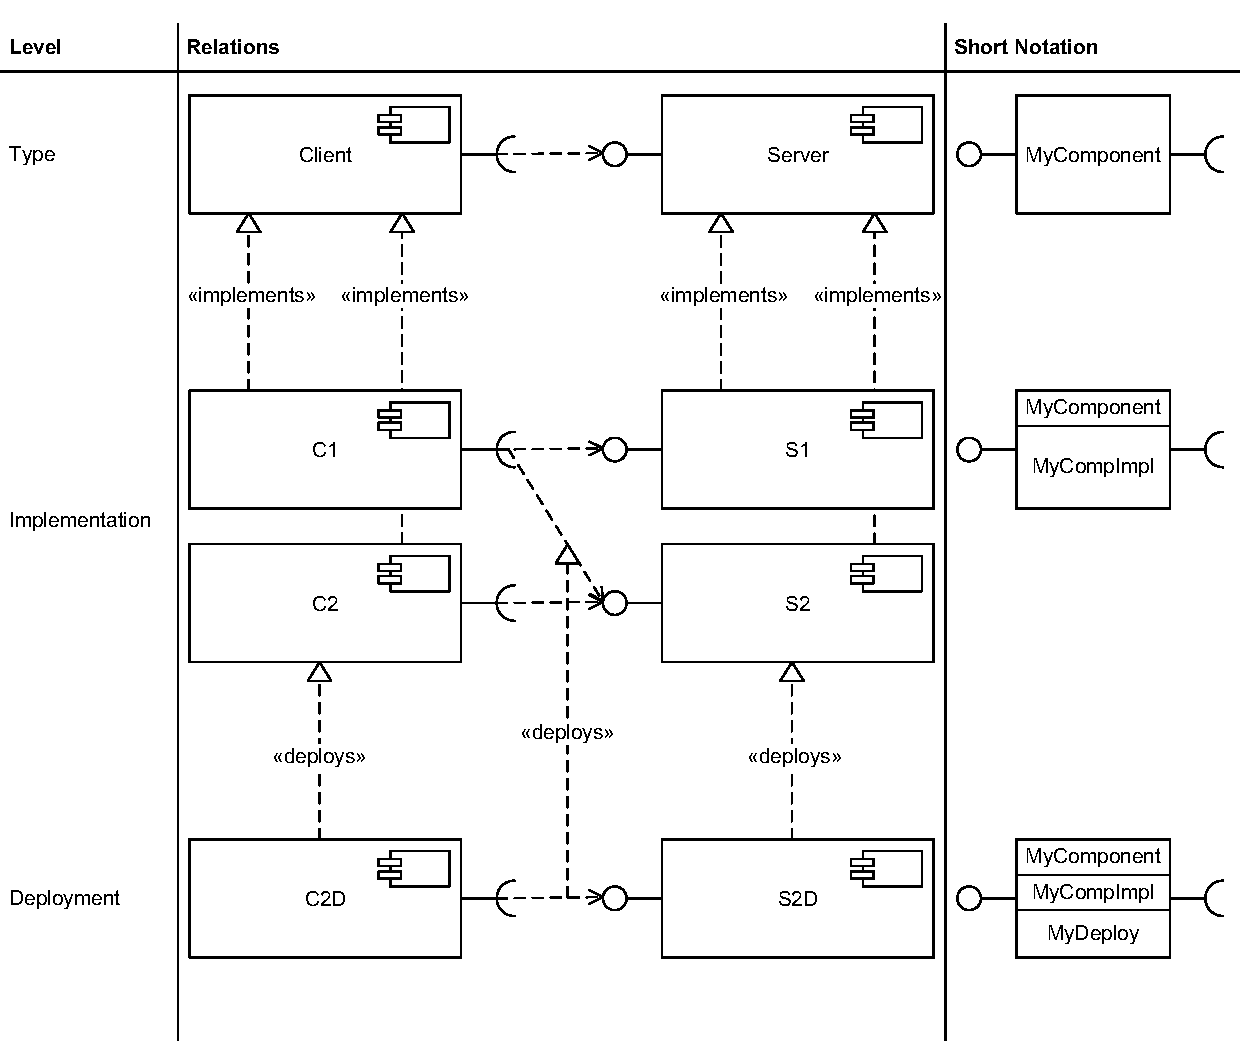
\includegraphics[width=1.00\textwidth]{images/level-example01.pdf}
	\caption{Example achitecture spread across the layers}
	\label{fig:level-example01}
\end{figure}

Figure \ref{fig:level-example01} shows a simple example how to visualize a component's architecture across the different levels of the component model. Especially the $\ll$deploys$\gg$-relation of connection from the implementation- to the deployment-level might be of interest, as here ressources can be assigned to connections.

The short notation allows to model, though only one level of the component model is displayed. By picking up the name of the inherited components from the higher levels it should be clear which type- or implementation-level component is currently worked with.



\subsection{Model}
\label{sec:Model}
The component model is realised as an abstract data type (ADT). This means that the data types have no methods except to modify the structure itself. So the component model is a pure data container for the architecutural informations and the entities attributes.

All entities are put to a relational scheme. So the component model consists of huge n-tuples that allow free navigation across the architecture. This way is has a kind of database-character for the set of entities, which provides a direct and quick access to attributes and entities. As well a central serialization can be executed on the objects.

Especially it is possible to have entities that are not connected to the rest of a architecture. Although these entities are not part of the entire model (because they are not part of the architecture), they can be caught. For the modeller this gives the possibility to design e. g. a set of components, that can be put to the architecture later on.

The whole component model is part of a kind of "super-entity", which is a central suspension for the model. This super-entity is offering a builder (according to the builder-pattern \cite{gamma}). Therefore building complex parts of the model is fully encapsulated to the model. This makes the creational process easier for users.

Furthermore the component model centrally "knows" which entities exists and may manage them (e. g. create, load, save, change-events). So the relational access to the entities and consistence-checks (see section \ref{sec:Consistence}) are monitored by the super-entity as well.

 

\subsection{Consistence}
\label{sec:Consistence}
\textit{External consistence-checks} are not part of the component model itself. As already explained above, the component model is a pure ADT. So consistence-mechanisms are performed through the "super-entity" using \textit{external} methods. This procedure allows to use different strategies (see the "strategie-pattern" in \cite{gamma}) for performing checks. As consistence might be defined quite differently no universal strategie is implemented in the model itself. External consistence-checks have to be started manually. This means that it is possible to build up models that do not fit to all available definitions of consistence. E. g. it is even possible to define contradicted checks, that can not be fulfilled at the same time. It might be easier to differ external consistence from internal consistence if it is called "\textit{validity}".

Validity-checks are imagineable for at least the following entities:

\begin{itemize}
	\item \emph{Protocols}: E. g. the accepted languages have to be subsets, or the protocols have to be exactly the same.
	
	\item \emph{Signatures}: E. g. the signaturelist has to be a subset, or the signaturelist needs to match exactly.
	
	\item \emph{QoS-attributes}: E. g. all attribute have to match, or a number of QoS-attributes has to fit.
	
	\item \emph{Connectors}: A strict definition might claim, that delegation connectors must be used between the same kinds of interfaces (required or provided), and assembly connector can be defined only between a provided and required interfaces that are directly compatible. Other validity-checks might define interfaces compatible if signatures and protocols are subsets ($provides\ interface \ \supseteq \ requires\ interface$). It should become clear that there is a broad field of possible definitions.
\end{itemize}

\textit{Internal consistence} is directly granted by model. This means that interfaces cannot be interconnected, or components have to use interfaces for connections. The model grants a valid architectural structure. Other constructions are not possible.



\subsection{Strategies}
\label{sec:Strategies}
Strategies are used for equals-checks as well. Possible strategies for equals-checks are:

\begin{itemize}
	\item \emph{Referencial}: The objects reference is checked (like it is default for equals in C\# or Java).
	
	\item \emph{GUID}: It is checked whether the GUIDs of two objects match.
	
	\item \emph{Deep}: E. g. composite components are recursively checked for identical signaturelists, implemented interfaces, roles, internal SEFFs and so on. Only if all subcomponents fit to objects / components are equal.
\end{itemize}

E. g. the equals strategie is used for hashtables as well. Only if the actual definition of equals meets objects are returned.






% ############################
\newpage
\section{Static Structure}
\label{sec:staticStructure}

\begin{quote}\emph{\emph{\textbf{ TODO: this section is not reviewed yet. }}}\end{quote}

The meta-model as described in the previous section is realised in a .NET assembly. The complete structure of the interfaces involved can be seen in figure \ref{fig:classdiagramm}.

\subsection{Components}

A central interface used here as entry point for the description is IComponent and its associates IBasicComponent and ICompositeComponent.

As one of the elementary concepts of component based software engineering is the compositionality of components, e.g., to build new applications and components from existing ones, the Palladio component model supports this by the composite design pattern. The relevant part of the class digram is shown in figure \ref{fig:compositecomponent}.

\begin{figure}[!ht]
	\centering
		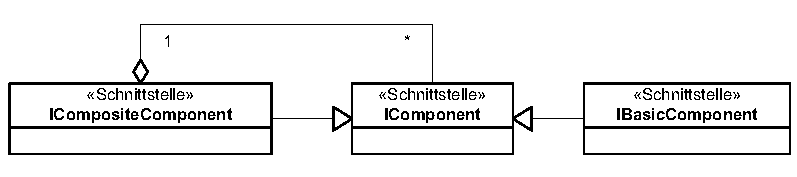
\includegraphics{images/composite-component01.pdf}
	\caption{The composite structure of the component model}
	\label{fig:compositecomponent}
\end{figure}

The abstraction of a basic and a composite component is the IComponet interface. Common to all components is their external representation. Therefore the IComponent interface supports editing a components provides and requires roles. The internal representation of a basic and a composite component are too different so that this aspect could not be added to the IComponent interface. 

Composite components consist of a non-empty set of IComponents which make up the composite component. In addition a composite component is responsible for managing the connections (provides-, requires-mappings and bindings) of the components.

Basic components are those components that can not be split any further in components either because they don't use other components or the internal structure is simply unknown. As these components can not be decomposed further it makes sense to associate service effect specifications to basic components. The reason for attaching service effect specifications to basic components and not to single interface specifications is that we don't want to restrict the implementer of a certain provides interface to an associated service effect. The amount of external dependencies a component has to its environment is part of the design decision when implementing a single basic component.

A basic component is therefore able to map a role identifier and a signature contained in this role to a service effect specification. The mapping is a 1 to 0..1 relationship as a service effect specification is \emph{optional}. Note that if an algorithm needs a certain kind of service effect specification it should assert first, that all the required information are specified!

\subsection{Interfaces}
\begin{figure}[htb]
	\centering
		%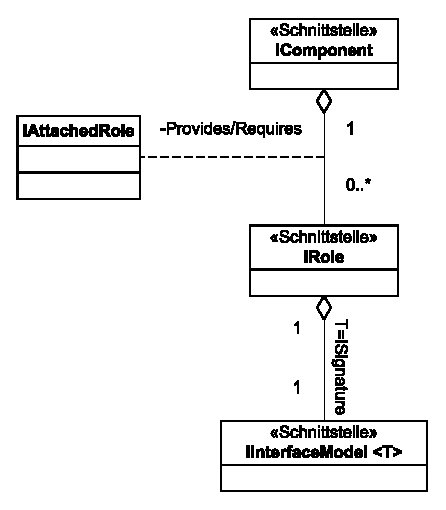
\includegraphics[scale=0.7]{pics/compinterface.eps}
	\caption{Components, Interface Models and Roles}
	\label{fig:compinterface}
\end{figure}

Associated to each component are two sets of roles: a set of provided roles and a set of required roles (see figure \ref{fig:compinterface}). The set of provided roles should have at least one element for being a valid component. Each role introduces an identifier unique to the component and has exactly one interface model associated to it (see below for a description of those). Important is that the association between a component and its role respectively the identifier of the role is a \emph{named} association called IAttachedRole which is used in an IConnection.

\subsection{Interface Model}
An important concept in the Palladio component model is the one of \emph{interface models} (see figure \ref{fig:intefacemodel}).

\begin{figure}[htb]
	\centering
		%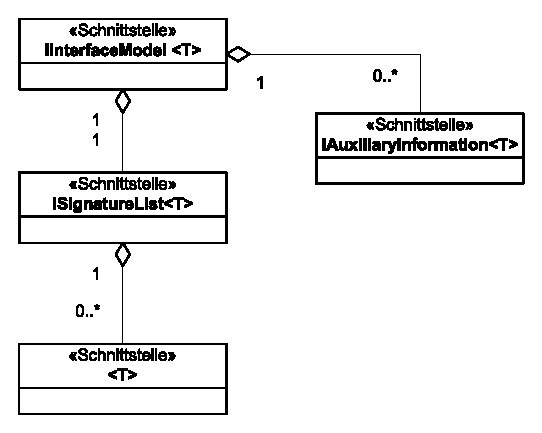
\includegraphics[scale=0.6]{pics/intefacemodel.eps}
	\caption{Interface Model}
	\label{fig:intefacemodel}
\end{figure}

An interface model is used to abstract away from the different approaches to specify rich interfaces. Rich interfaces are those having more information than only a list  of signatures of the services of the respective interface. Additional, or like it is called here, auxiliary information can contain protocol specifications, i.e., protocol FSMs, petri-nets, pre- and postconditions, re-entrance specifications, QML contracts, ... As today's component technologies only support signature list based provides interface specifications only the signature list is mandatory. Any other (more or less scientific) auxiliary specification data can be attached according to the algorithms needed in a specific context. 

There is a resulting problem with this concept. For the auxiliary information it might be important to check the consistency of the specification data. But the consistency depends on the checking if the signatures in the auxiliary specification are part of the signatures contained in the signature list. Therefore the component model uses an observer pattern on the signature list to inform the auxiliary specification objects about changes on it. The FSM protocol auxiliary specification uses this concept for example to automatically adjust the FSM's input alphabet to be identically to the signatures in the signature list. The observer pattern is implemented by using the .NET event mechanism, the necessary delegates can be found in the main namespace. As the usage of this concept can't be enforced by the type system, please read the respective code documentation before creating a new auxiliary specification object.

An other important concept is the usage of a \emph{generic} interface model. The generic type parameter is a place holder for the type of the signature contained in the signature list. As described in the introduction there are two types of signatures: internal signatures which are part of a certain interface and external signature referencing services outside of the containing component. The problem with this idea is that support for generic data types is initially introduced in C\# 2.0 which is not yet available. Therefore at present we use code generator for the generation of the strongly typed container types. As this is not very handy, we hope that at least a beta version of C\# 2.0 is available soon so that we can update the code base to use real generics.

\subsection{Signatures}
Signatures are modelled as depicted in figure \ref{fig:signatures}. 

\begin{figure}[htb]
	\centering
		%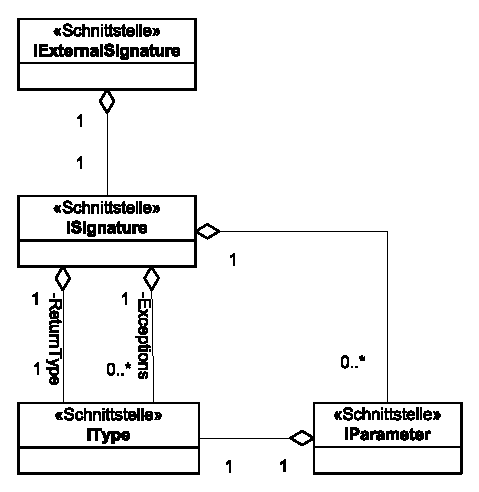
\includegraphics{pics/signatures.eps}
	\caption{Signaturen}
	\label{fig:signatures}
\end{figure}

There is nothing unusual about this. A signature is characterised by a return type, an identifier, an ordered list of parameters and an unordered list of exceptions (note that exceptions are not part of the standard interface/signature model in .NET). Additionally, as noted in the introduction there are external signatures consisting out of a role and a signature (the association to the role can be seen in figure \ref{fig:classdiagramm}).

\subsection{Connections}

Connections are part of composite components and are used to connect roles of components. They are modelled as depicted in figure \ref{fig:connection}. 

\begin{figure}[htb]
	\centering
		%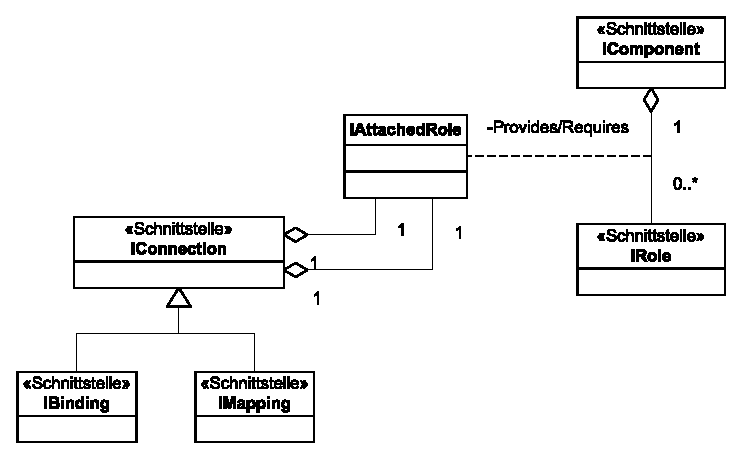
\includegraphics[scale=0.95]{pics/connection.eps}
	\caption{Connections, Mappings and Bindings}
	\label{fig:connection}
\end{figure}

There are two specializations of a connection: binding and mapping (see also figure \ref{fig:connections}). Bindings connect required roles to provided roles in order to fulfill the need for service. Mappings are only logical connections between the outer interfaces of a composite component and the inner ones. A connection always runs from a requiring role to a providing one (in the case of mappings this might sound a bit strange, but just imagine the outer interfaces having a mirror interface to the inside of a composite component). One important aspect of connections is, that it is assumed that a connection is valid with respect to the services required and provided, e.g., that every required service can be found exactly on the provides role. Renamings, parameter changes, overload resolving and the like is not done along a connection. If it is necessary to introduce such things one has to introduce an adaptor for these tasks.

\subsection{Full static structure}

The complete structure is depicted in figure \ref{fig:classdiagramm}.

\begin{figure}[htb]
	\centering
		%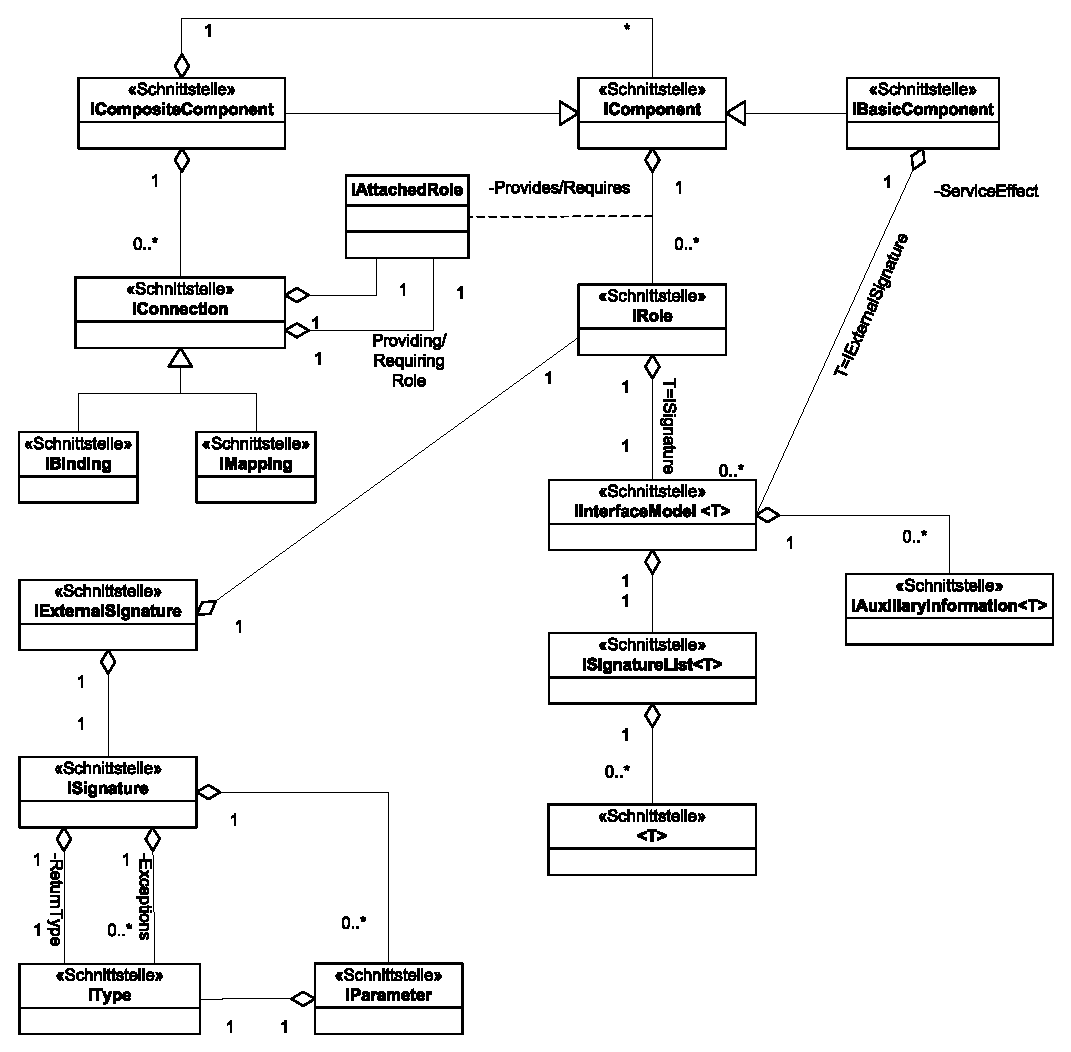
\includegraphics[scale=0.95]{pics/classdiagramm.eps}
	\caption{Full Class Diagramm of the Palladio Component Model}
	\label{fig:classdiagramm}
\end{figure}




\bibliographystyle{ieeetrans}
\bibliography{quellen}


\end{document}
